\documentclass[10pt, letterpaper]{article}
\usepackage{graphicx}
\graphicspath{{images/}} 
\usepackage{titling}
\usepackage{amsmath}
\usepackage{listings}
\usepackage{xcolor}
\lstset{language=Matlab,%
    basicstyle=\footnotesize\ttfamily,%
    breaklines=true,%
    keywordstyle=\color{blue},%
    identifierstyle=\color{black},%
    stringstyle=\color{myorange},%
    commentstyle=\color{mygreen},%
    showstringspaces=false,%without this there will be a symbol in the places where there is a space
    numbers=left,%
    numberstyle={\tiny \color{black}},% size of the numbers
    numbersep=9pt, % this defines how far the numbers are from the text
    emph=[1]{for,end,break},emphstyle=[1]\color{red}, %some words to emphasise
    %emph=[2]{word1,word2}, emphstyle=[2]{style},    
}

\usepackage[margin=1in]{geometry}
%\setlength{\droptitle}{-12em}
\title{
\vspace{10pt}
\hrule
\vspace{15pt}
\textbf{Transient Circuit Analysis with Laplace
Transform}
}
\author{Hamza Siddiqui \\ 400407170 \\ siddih38}
\date{\today 
\vspace{15pt}
\hrule
\vspace{350pt}

\includegraphics[width=0.3\textwidth]{images/mac.png}
}
\begin{document}
\maketitle
\newpage
\section*{\textbf{Exercise 1:} \textbf{Transient 1\textsuperscript{st}
 Degree Circuit Analysis with LT}}

\begin{enumerate}
\item \textbf{Complete Schematic:} Include the complete schematic (screenshot or image export).  

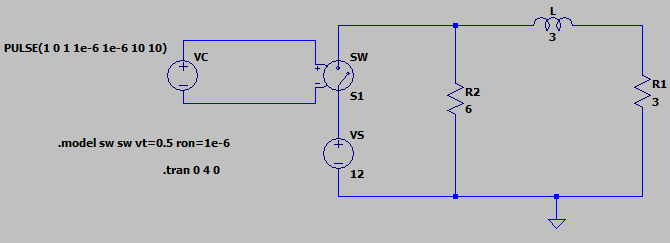
\includegraphics[width=0.9\textwidth]{images/circuit1.png}

\item \textbf{Complete Netlist:} Include the complete netlist (View→SPICE Netlist). 
\begin{verbatim}
* C:\Users\hamza\OneDrive\Documents\2cf3\assignment 4\exercise1.asc
VC N003 N004 PULSE(1 0 1 1e-6 1e-6 10 10)
S1 N005 N001 N003 N004 SW
VS N005 N006 12
L N001 N002 3
R1 N002 N006 3
R2 N001 0 6
.model sw sw vt=0.5 ron=1e-6
.tran 0 4 0
.backanno
.end
\end{verbatim}

\item \textbf{Simulation Plot: }Include the plot of $V_C(t)$ and $i(t)$ from the LTspice simulation.

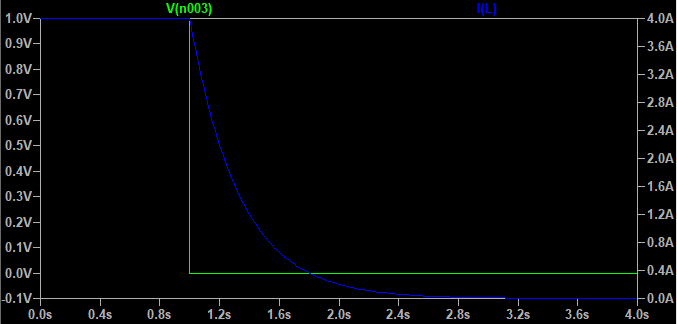
\includegraphics[width=0.9\textwidth]{images/ltplot1.png}

\item \textbf{Analytical Solution: }Include your analytical solution for $i(t)$ based on the Laplace transform.

\textit{Deriving time-dependent current through the inductor branch using s-domain analysis:} 

For the initial condition, prior to opening the switch, the circuit is in steady-state, hence the inductor acts as a short circuit. This results in the initial current to be 4 A:
\begin{align*}
    i(t = 0_-) &= \frac{12}{3} \\
               &= 4 \ \text{A}
\end{align*}

Then, s-domain analysis can be used to determine $i(t)$. With the now open, the circuit simply becomes the following network:
\begin{center}
    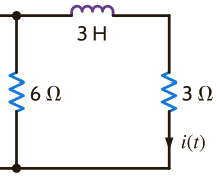
\includegraphics[width=0.2 \textwidth]{images/OC1.png}
\end{center}

Applying Kirchhoff's Voltage Law, we can compute as follows:

\begin{align*}
    (6+3) i(t) + L \frac{dI}{dt} &= 0 \\
    \text{Applying Laplace Transform: } \\
    9\ i(s) + Ls\ i(s) - Li(0_-) &= 0 \\ 
    9\ i(s) + 3s\ i(s)            &= 3\times 4 \\
    9\ i(s) + 3s\ i(s)            &= 12 \\
    i(s) &= \frac{12}{9+3s} \\
        &= \frac{4}{s+3}
\end{align*}
Then by taking the inverse Laplace transform to solve for the circuit response in the time domain, we get the final result: \\
$$ i(t) = 4 e^{-3t} u(t) \ \text{A}$$ 

\item \textbf{MATLAB code and plot: }Include the MATLAB source code and plot in your PDF report.

MATLAB source code: 
\begin{lstlisting}
clear all; close all; % clean up memory and close all open plot windows
t = linspace(0, 1, 1001); % vector of time samples where function is calculated
i = 4*exp(-3*t);
figure;
plot(t, i);
grid on;
title('Current through Inductor in Exercise 1');
xlabel('{\it t} (s)');
ylabel('{\it i} (A)');
\end{lstlisting}
\newpage
Obtained MATLAB plot: 
\begin{center}
    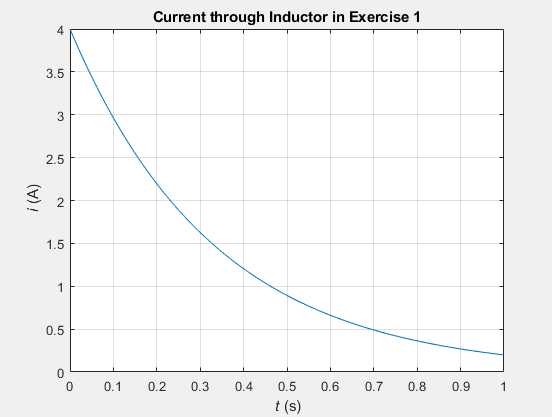
\includegraphics[width=0.7\textwidth]{images/mlplot1.png}

\end{center}

\item \textbf{Observations: }Does the LTspice simulation result agree with the MATLAB plot of the theoretical result? Justify
your answer.

The two plots agree with each other as seen through the initial condition being noticeable in both figures - that being an initial branch current of 4 A. Furthermore, they are both decreasing exponentially, which is the obvious expectation for an exponentially decreasing function obtained for current. The LTSpice simulation plot is simply shifted by 1s as a result of the inclusion of the circuit's behaviour prior to the switch being opened. The switch is opened at t = 1s, and once it is opened, the plot demonstrates the current in the inductor exponentially decreasing until it reaches steady-state that extends to infinite time ($4\times e^{-3\times \infty} = 0$). This is a result of the PULSE configuration that sets the voltage to stay at 0 V after switching for a time longer than the simulation time of 4.0s. The voltage trace is added on the same plot to explain this shift. The MATLAB plot begins from when we open the switch, and so at time t= 0s, the exponential coefficient simply becomes 1, and the initial condition is seen starting at 0s with no shift involved. 

\end{enumerate}
\newpage    
\section*{\textbf{Exercise 2:} \textbf{Transient 2\textsuperscript{nd}
 Degree Circuit Analysis with LT}}
 \begin{enumerate}
\item \textbf{Complete Schematic:} Include the complete schematic (screenshot or image export).  

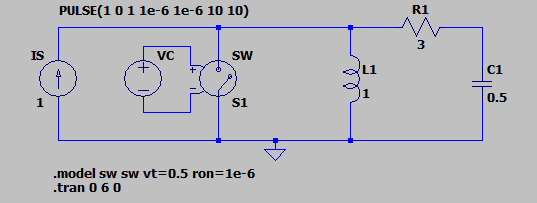
\includegraphics[width=0.9\textwidth]{images/circuit2.png}

\item \textbf{Complete Netlist:} Include the complete netlist (View→SPICE Netlist). 
\begin{verbatim}
* C:\Users\hamza\OneDrive\Documents\2cf3\assignment 4\exercise2.asc
IS 0 N001 1
S1 0 N001 N003 N004 SW
VC N003 N004 PULSE(1 0 1 1e-6 1e-6 10 10)
L1 N001 0 1
C1 N002 0 0.5
R1 N002 N001 3
.model sw sw vt=0.5 ron=1e-6
.tran 0 6 0
.backanno
.end
\end{verbatim}

\item \textbf{Simulation Plot: }Include the plot of $i_L(t)$ and $i_C(t)$ from the LTspice simulation.

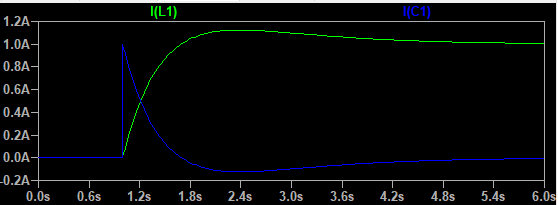
\includegraphics[width = 0.9\textwidth]{images/lt2.png}

\item \textbf{Analytical Solution: }Include your analytical solution for $i_L(t)$ and $i_C(t)$ based on the Laplace transform.

Using the fact that $$i_C(t) + i_L(t) = \frac{1}{s} $$ and $$ V_C(t) + V_R(t) = V_L(t),$$
We can substitute $i_L(t) &= \frac{i_C(s)}{sL}(R+\frac{1}{sC}) $ into the equation to obtain the following: 

\begin{align*}
   i_C(s) &=  \frac{1}{s} - \frac{i_C(s)}{sL}(R+\frac{1}{sC}) \\
          &= \frac{s}{s^2 + 3s + 2} \\
  i_C(t) &= (2 e^{-2t} - e^{-t}) u(t)\ \text{A}
\end{align*}
Therefore, 
\begin{align*}
    i_L(s) &= \frac{3s+2}{s(s+2)(s+1)} \\
    i_L(t) &= (e^{-t} -2e^{-2t} + 1)u(t) \ \text{A}
\end{align*}
\item \textbf{MATLAB code and plot: }Include the MATLAB source code and plot in your PDF report.

MATLAB source code: 
\begin{lstlisting}
clear all; close all;
t = linspace(0, 1, 1001);
iL = exp(-t) -2*exp(-2*t) + 1;
iC = 2*exp(-2*t) - exp(-t);
figure;
plot(t, iL,'-k') % plot curve in solid black line
hold on;
plot(t, iC,'--b') % plot curve in dash blue line
hold off;
grid on;
legend('{\it i}_L','{\it i}_C')
title('Currents in Exercise 2')
xlabel('{\it t} (s)');
ylabel('{\it i} (A)');
\end{lstlisting}
Obtained MATLAB plot: 
\begin{center}
    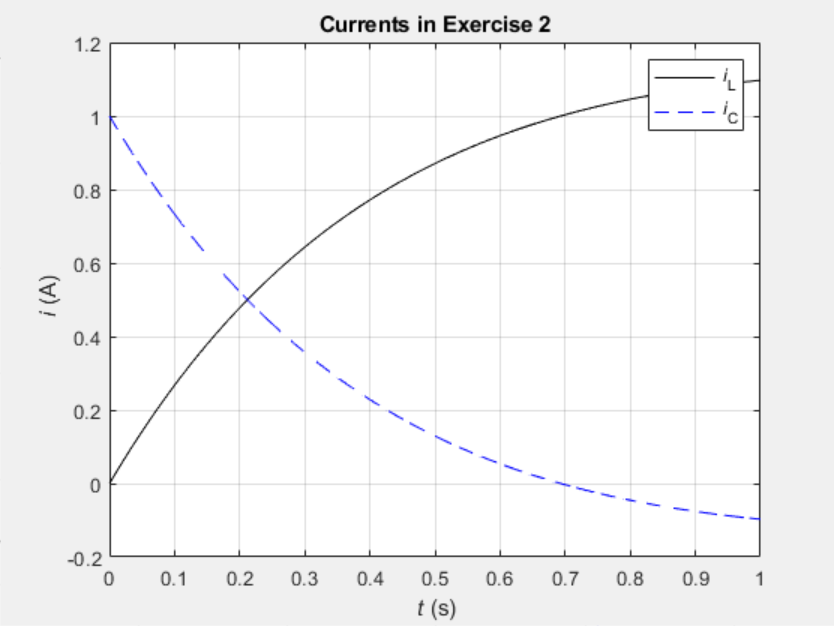
\includegraphics[width=0.7\textwidth]{images/ml2.png}
\end{center}
\newpage
\item \textbf{Observations: }Does the LTspice simulation result agree with the MATLAB plot of the theoretical result? Justify
your answer.

It is evident that both the LTSpice simulation plot and the MATLAB plot agree with one another. In the LTSPice plot, the behaviour is displayed for one second prior to the state switch, hence it is shifted one second ahead relative to the MATLAB plot. When observing the transient states in both plots, the behaviours agree with each other for both currents that are plotted. Relevant points here are the starting the points, which are 1A and 0A respectively for current through the capacitor and inductor (realized in both plots), and the asymptotic behaviour as $t \rightarrow \infty$, which reaches back to steady state for both currents shown in both plots, though more noticeable in the LTSpice plot.
\end{enumerate}
\end{document}